\documentclass[a4paper]{scrreprt}

\usepackage{scrhack}
\usepackage{graphicx}
\usepackage[utf8]{inputenc}

\addtokomafont{titlehead}{\flushright}
\addtokomafont{subject}{\vspace{3cm}\flushleft}
\addtokomafont{title}{\flushleft}
\addtokomafont{subtitle}{\flushleft}
\addtokomafont{author}{\flushleft\setlength{\tabcolsep}{0pt}}
\addtokomafont{date}{\flushleft}
\addtokomafont{publishers}{\flushleft}

\titlehead{
\includegraphics[scale=2]{../templates/logo_en}}
\subject{Software Engineering and Design}
\title{Requirements Specification}
\subtitle{Mental Health Care Patient Management System (MHC-PMS)}
\author{
\begin{tabular}{l}
\normalfont\bfseries{Team White:}\\
Dellsperger Jan\\
Ellenberger Roger\\
Sheppard David\\
Sidler Matthias\\
Spring Mathias\\
Thöni Stefan
\end{tabular}
}
\date{\today}
\publishers{Version 1.0}

\begin{document}

\begin{titlepage}
	\maketitle
\end{titlepage}


\tableofcontents


\chapter{Vorwort}
% This should define the expected readership of the document and describe its version history, including a rationale for the creation of a new version and a summary of the changes made in each version.


\section{Über dieses Dokument}
Dieses Dokument beschreibt den Requirements-Engineering-Prozess des Projekts \textit{MHC-PMS}. Es spezifiziert die Erkenntnisse auf dem Design-Thinking-Prozess.


\section{Zielgruppe}
Das Dokument richtet sich an den Endkunden, die Projektleitung, die Personalplanung, die Entwickler, Test-Engineers und das zukünftige Betriebsteam.


\section{Änderungsnachweis}
\begin{table}[h]
\label{tab_version-history}
\begin{tabular}{llll}
{\bf Version} & {\bf Beschreibung} 							& {\bf Autor} 	& {\bf Datum} \\
0.1         & Dokument aus Vorlage erstellt 				& Team White 		& April 1, 2016  \\
1.0         & Finale Version des Dokuments					& Team White 		& \today  \\



\end{tabular}
\end{table}



\chapter{Einleitung}
% This should describe the need for the system. It should briefly describe the system’s functions and explain how it will work with other systems. It should also describe how the system fits into the overall business or strategic objectives of the organization commissioning the software

Die Betreuung von Personen mit psychischen Störungen soll mit unserer Software vereinfacht werden. Die Zielkundschaft sind kleine bis grosse Einrichtungen für die Behandlung (ambulant und Hausbesuche) von Patienten mit psychischen Störungen.

Wir fokussieren dabei auf Funktionen für das Management. Wir möchten Personen mit Führungsfunktion bei Planungsarbeiten, administrativen Tätigkeiten und Strategie-Entscheidungen unterstützen. Die Verwaltung und Auswertung von Patientendaten (Behandlungshistorie und Verrechnung) steht dabei im Fokus. Zudem soll die Personalplanung mit der Patientenverwaltung verknüpf werden. Export von Berichten für Partnerorganisationen und Behörden soll möglichst unkompliziert gestaltet werden.

\bigskip

Unser Produkt ist rein für die Datenauswertung gedacht. Als Datenquellen nutzen wir eine bestehende Patientenverwaltung (mit Personalplanung und Verrechnung). Durch die gewonnen Erkenntnisse soll das Management ihre Strategie mit Fakten fundiert steuern können und im Alltag weniger administrativen Aufwand vorfinden. In er Gesundheitsbranche sollen damit Kosteneinsparungen erreicht werden. Ineffiziente Behandlungsarten können schneller erkannt und Patienten mit schlechten Behandlungserfolg besser überwacht werden.



\chapter{Glossar}
\begin{table}[h]
\label{tab_glossar}
\begin{tabular}{llll}
{\bf Begriff} 		& {\bf Beschreibung} \\
Dashboard			& Übersichtseite zu einem Themenbereich \\

HIT 				& Health IT: Informatik-Sparte, die sich mit dem Gesundheitswesen auseinandersetzt \\

MHC-PMS 			& Mental Health Care Patient Management System \\
DBS 				& Database System \\
Report				& Bericht / Auswertung


\end{tabular}
\end{table}




\chapter{User-Requirements Definition}
% Here, you describe the services provided for the user. The nonfunctional system requirements should also be described in this section. This description may use natural language, diagrams, or other notations that are understandable to customers. Product and process standards that must be followed should be specified. (Use Case- and Activity Diagrams)
Nachfolgender Abschnitt beschreibt die User-Requirements der Applikation.


\section{User Requirements}
Folgendes Diagramm zeigt die Use-Cases der Applikation.

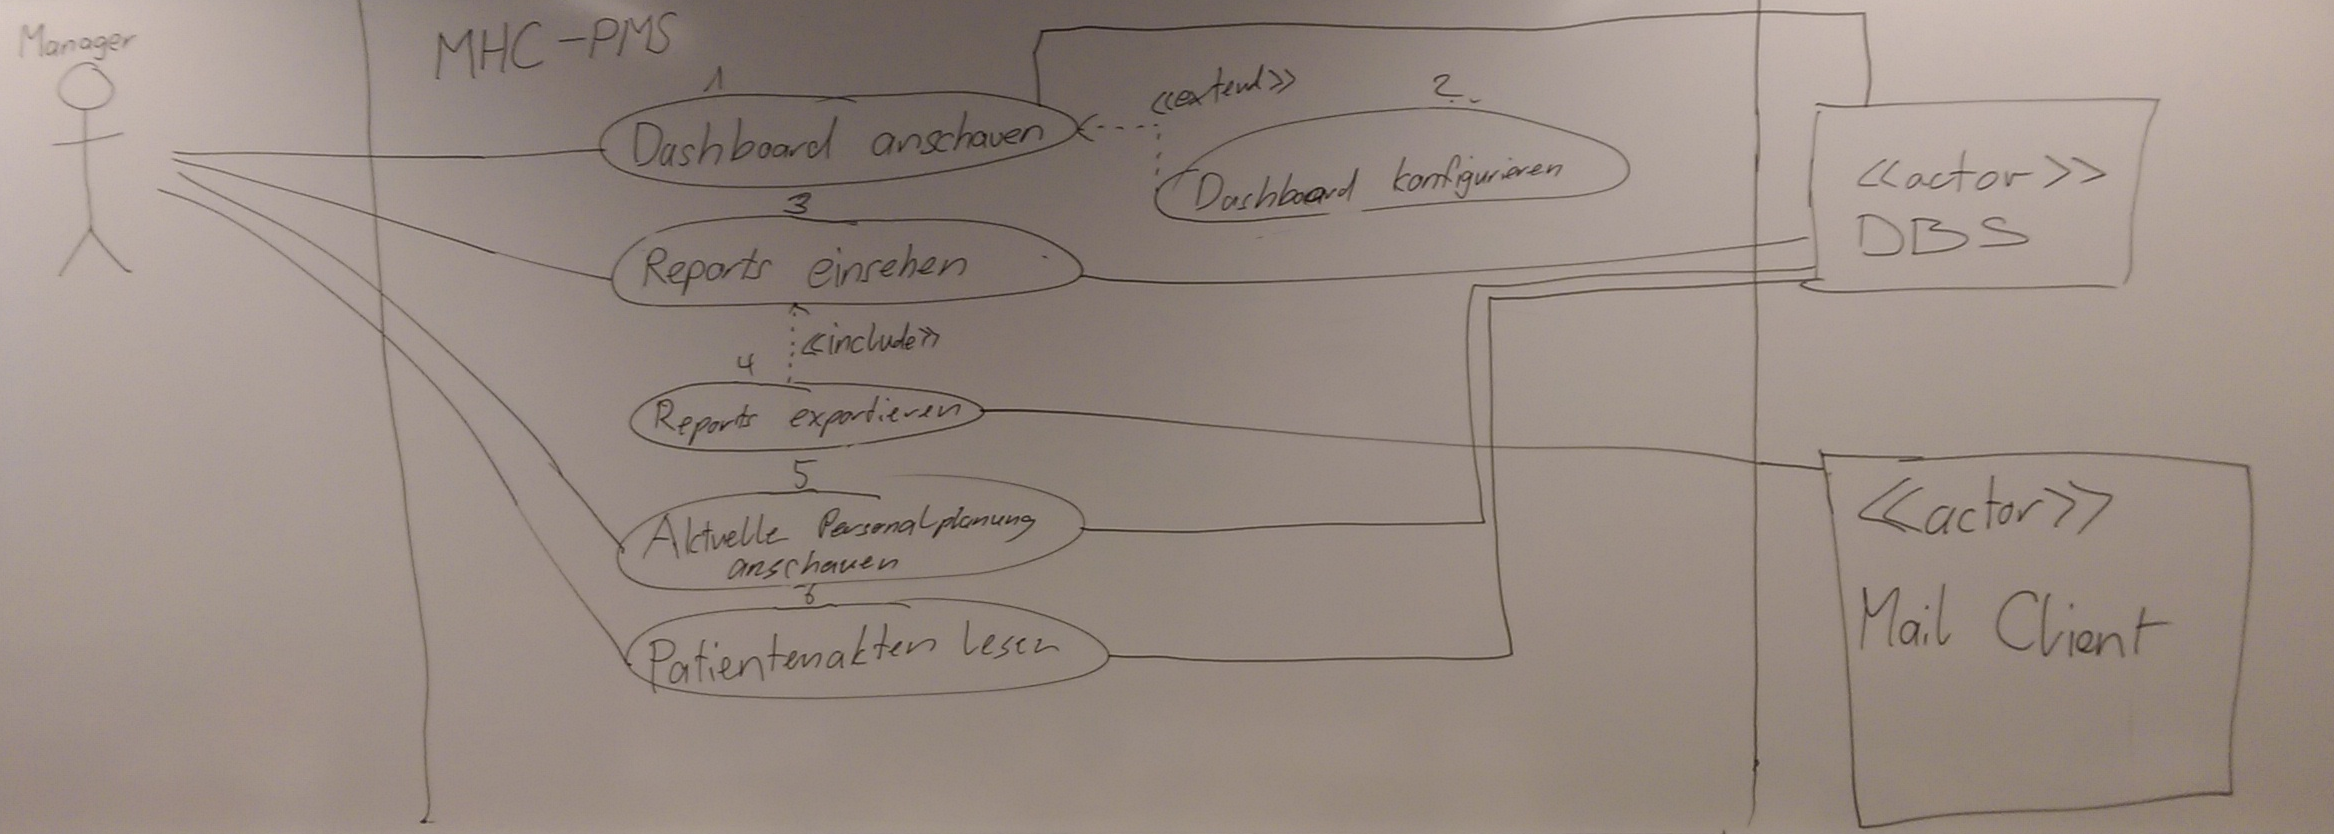
\includegraphics[width=1\textwidth]{img/use_case_diagram_20160401.png}

\bigskip

Es existieren sechs Use-Cases, wo der Benutzer mit dem System interagiert:
\begin{enumerate}
\item \textbf{Dashboard anschauen:} Daten werden aufbereitet und auf dem Dashboard angezeigt
\item \textbf{Dashboard konfigurieren:} Manager personalisiert sein persönliches Dashboard je nach Anforderungen individuell
\item \textbf{Reports einsehen:} Manager lässt Report zur Einsicht generieren
\item \textbf{Reports exportieren:} Generierte Reports werden zum digitalen Versand, Ausdruck oder lokalen Abspeichern exportiert.
\item \textbf{Aktuelle Personalplanung anschauen:} Manager sieht aktuelle Personalplanung an
\item \textbf{Patientenakten lesen:} Manager sieht Patientenakten ein
\end{enumerate}

Es existieren zudem zwei weitere Aktoren. Zum einen der zum Versenden der Reports benutzte Mail-Client, der auf den Endgerät vorausgesetzt wird, und ein Datenbanksystem "DBS" (oder allenfalls mehrere Datenbanksysteme) als Datenquelle.

\bigskip

Nachfolgend sind Use-Case eins und drei noch genauer beschrieben.


\pagebreak

\section{Use-Case 1}
\textbf{Aktivitätsdiagramm}

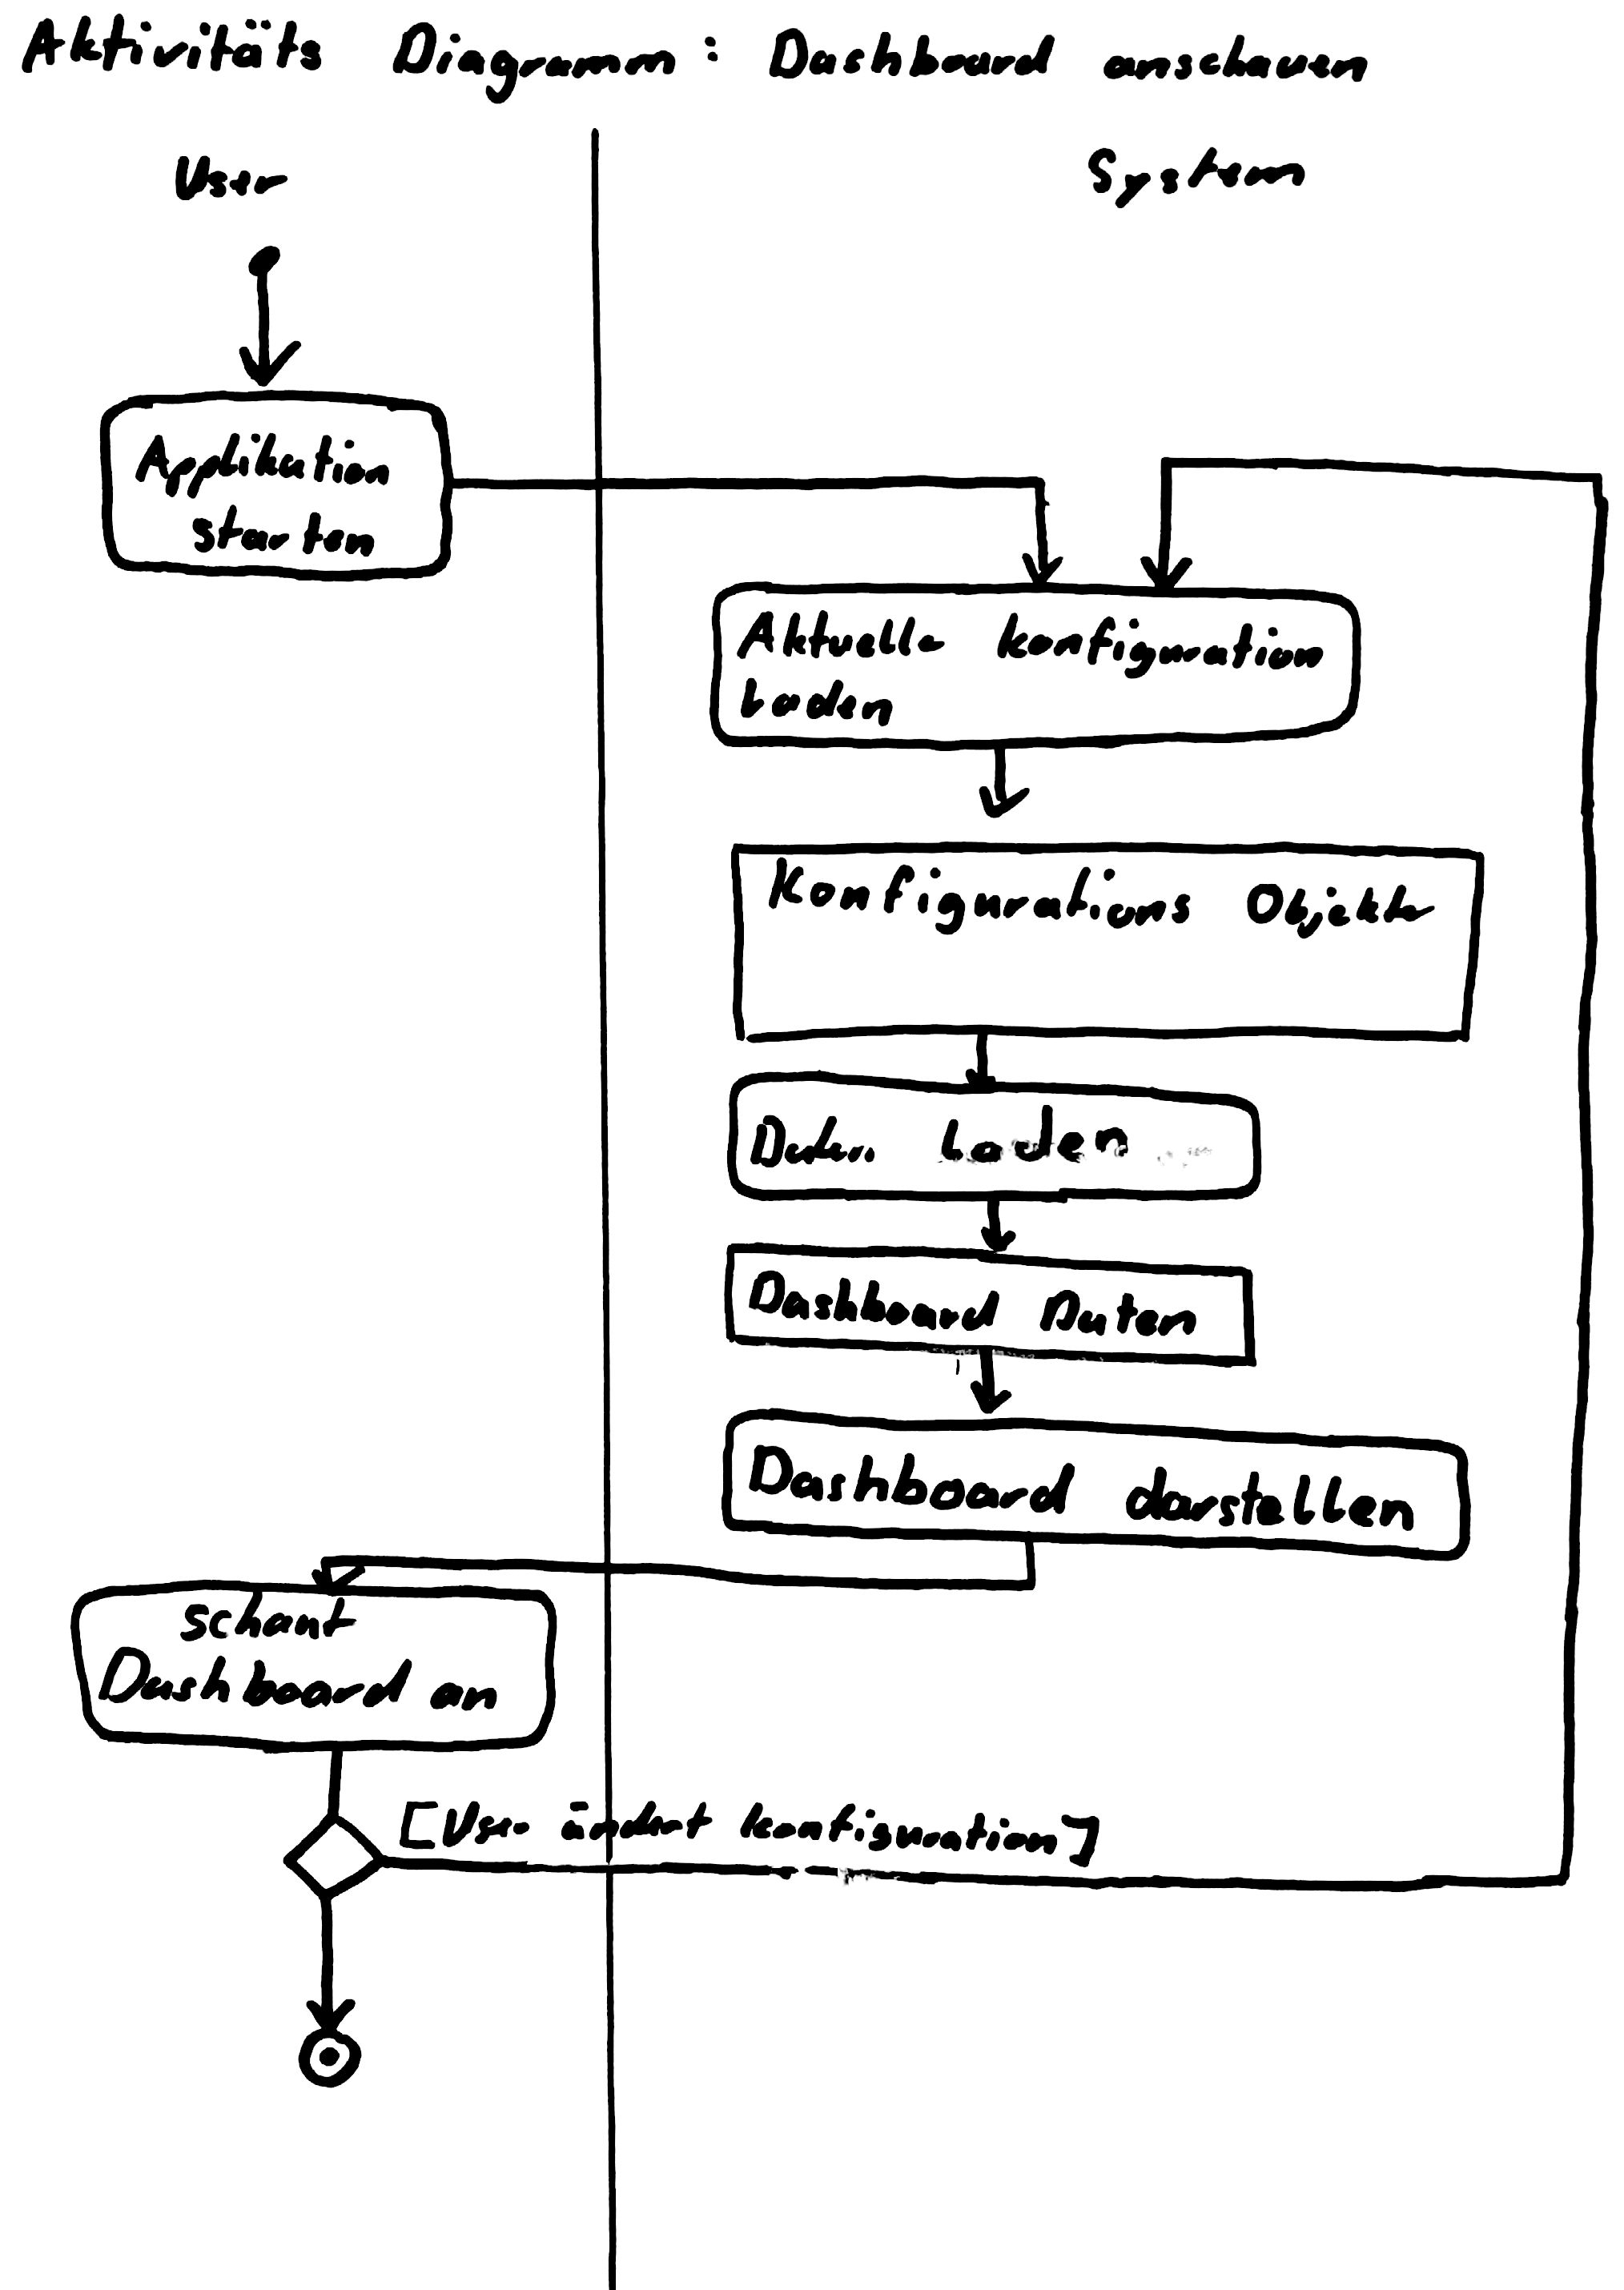
\includegraphics[width=0.9\textwidth]{uc-1_Dashboard/uc1_activity.jpg}


\pagebreak


\textbf{Szenario}

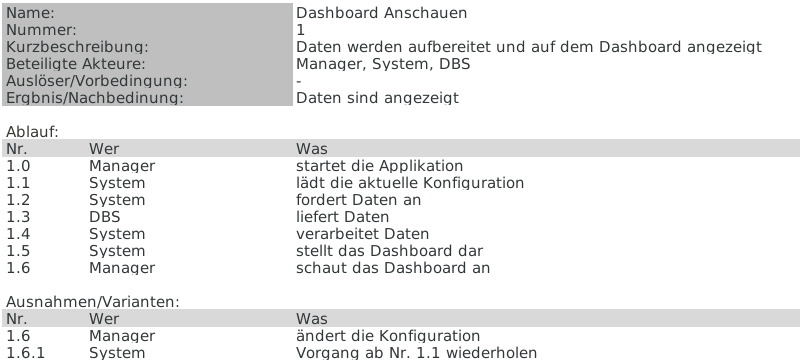
\includegraphics[width=1\textwidth]{uc-1_Dashboard/uc1_scenario.png}




\section{Use-Case 3}

\textbf{Aktivitätsdiagramm}

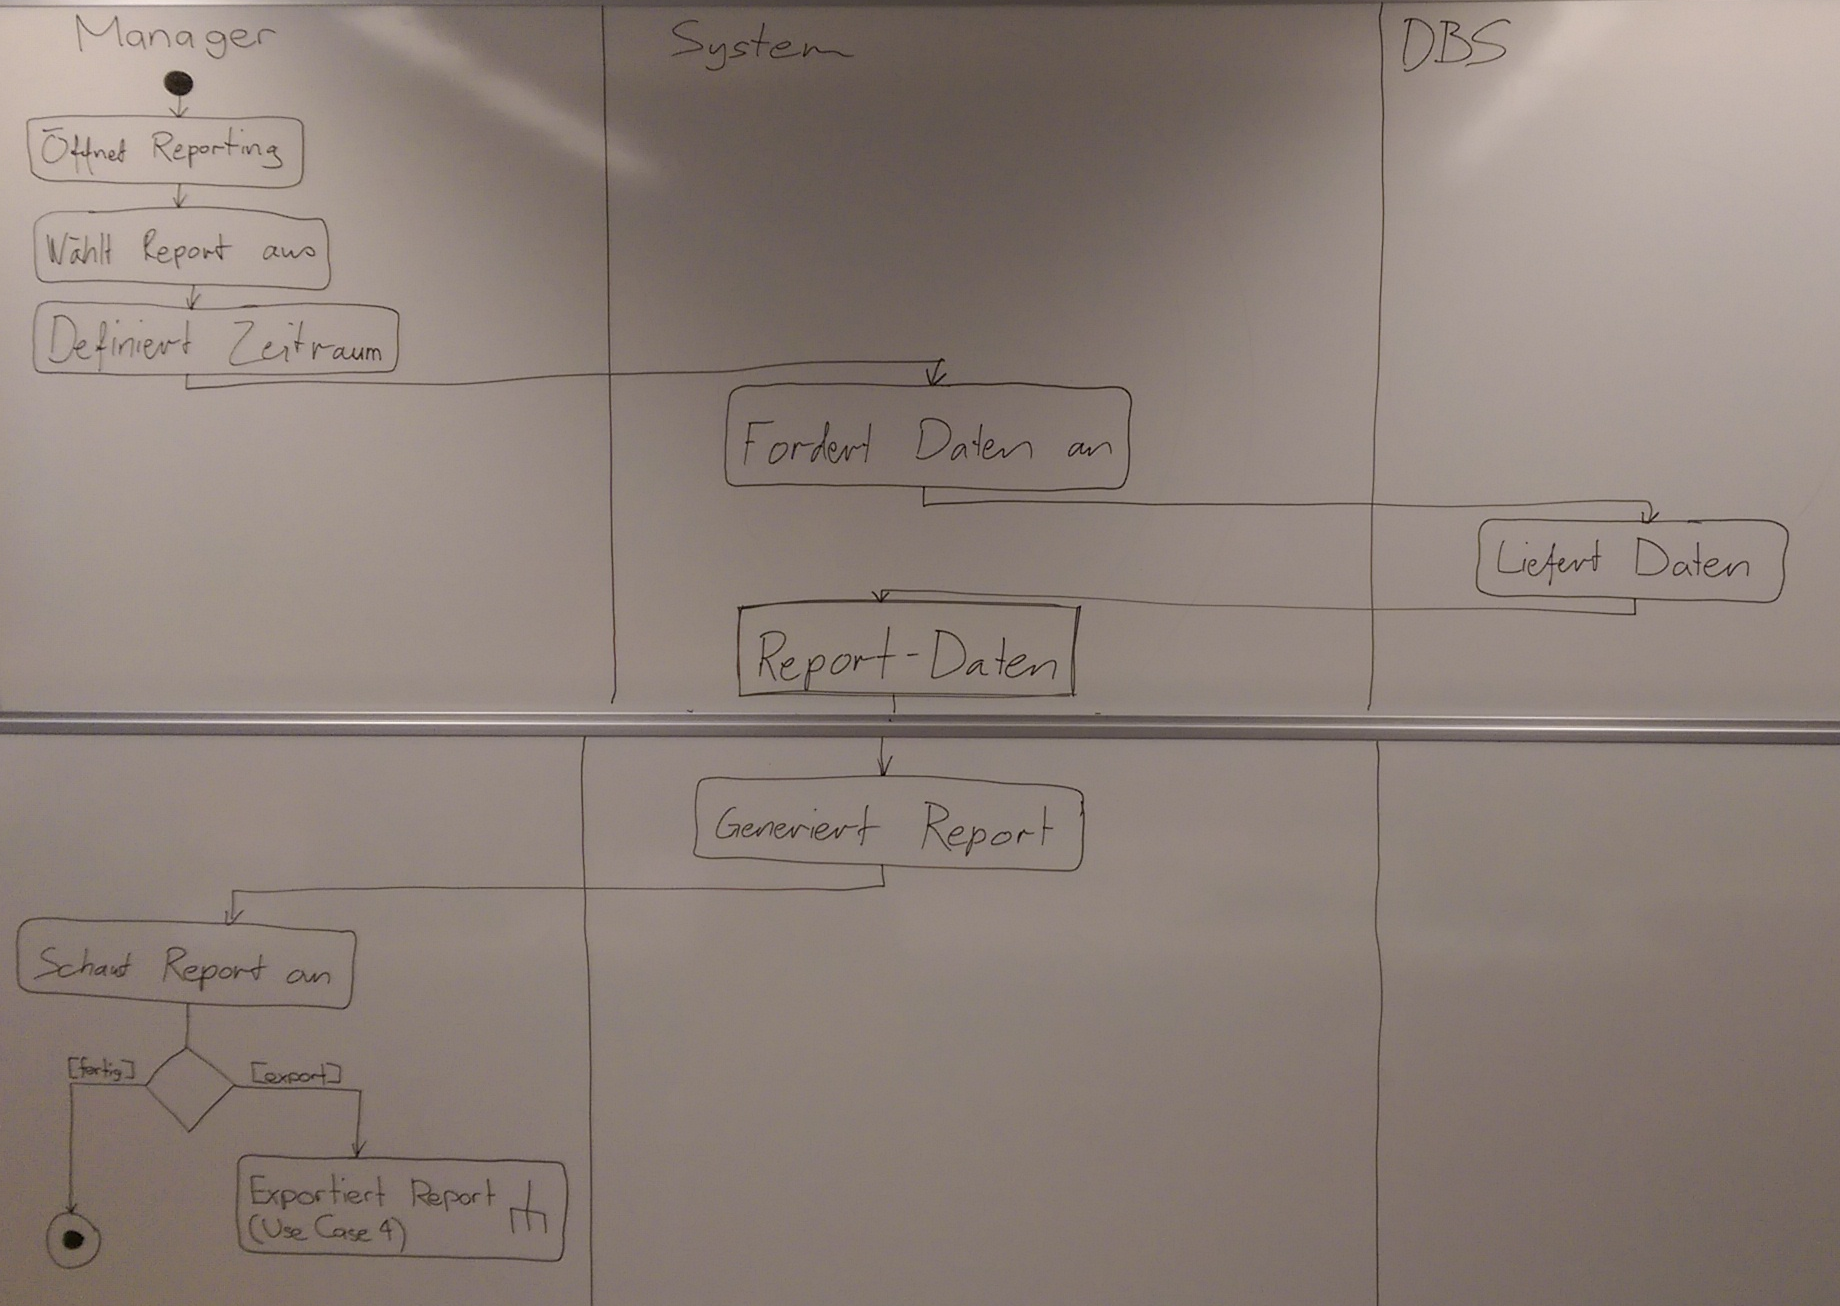
\includegraphics[width=0.9\textwidth]{uc-3_Report_einsehen/uc3_activity_diagram.png}

\pagebreak

\textbf{Szenario}

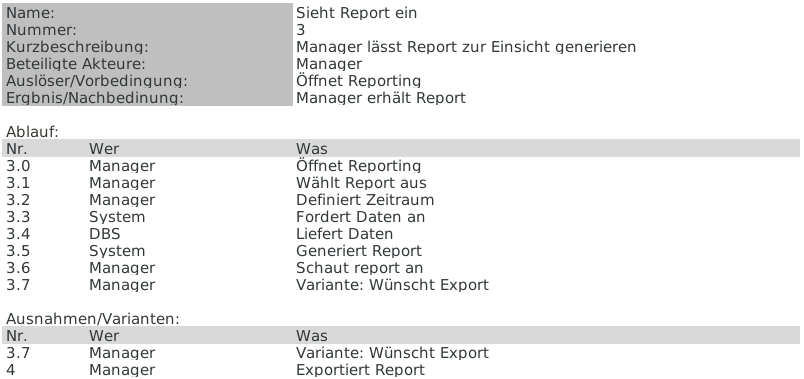
\includegraphics[width=1\textwidth]{uc-3_Report_einsehen/uc3_scenario.png}




\chapter{System Architektur}
Bei der Applikation handelt es sich um eine Webanwendung, welche für mobile Endgeräte optimiert ist. Ein gutes Benutzererlebnis soll aber auch auf anderen Endgeräten wie PCs oder Notebooks gewährleistet sein. Die Applikation befindet sich in einer isolierten Applikationslandschaft mit ledigilich einem DBS als Umsystem. Als Rahmenbedingung wird angenommen, dass dieses DBS alle Daten liefern kann, welche von Requirements verlangt werden.

\chapter{System-Requirements Spezifikation}

\section{Functional Requirements}
\subsection{UC1: Dashboard}
\paragraph{[1.1] Darstellung Dashboard}
Das System soll beim Starten oder alternativ per Klick auf ein Menu-Punkt ein Dashboard anzeigen. Dieses Dashboard soll, in Kacheln dargestellt, konfigurierte Kennzahlen und Statistiken darstellen. (Siehe Requirement [1.6]) Desweiteren soll per Klick auf einen solchen Kachel der entsprechende Report angezeigt werden. 
 	
\paragraph{[1.2] Dashboard Konfiguration}
Das System soll einen Menu-Punkt zur Verfügung stellen, der die Konfiguration des Dashboards erlaubt. Dies beinhaltet: 
\begin{itemize}
\item Wieviele Kacheln dargestellt werden (Bis zu einem Maximum von 6).
\item Welche Kennzahlen/Statistiken in Kacheln dargestellt werden.
\item In welcher Reihenfolge diese angezeigt werden
\end{itemize}

\subsection{UC3: Reporting}
\paragraph{[1.3] Reporting anzeigen}
Das System soll via Menu-Punkt eine Reporting Funktionalität anbieten. Dazu wird eine Art Wizard gestartet, der in folgenden Schritten zum Report führt:
\begin{enumerate}
\item \textbf{Reporttyp wählen:} Gemäss den Kennzahlen kann jeweils ein Report erstellt werden (Siehe Requirement [1.6])
\item \textbf{Zeitraum wählen:} Der Zeitraum kann frei gewählt werden. Insbesondere soll es möglich sein, individuelle Perioden (beispielsweise Quartal oder halbjährlich) zu definieren.
\item (Optional) \textbf{Weiteren Zeitraum hinzufügen:} Falls Zeiträume verglichen werden sollen, besteht hier noch die Option, eine weitere Periode hinzuzufügen.
\end{enumerate}
Danach wird die Grafik angezeigt und in einer zweiten View die Primärdaten tabelarisch aufgelistet. Zwischen diesen Views kann zum Beispiel mit einer Swipe Geste oder Menu Buttons gewechselt werden. Falls einen weiteren Zeitraum ausgewählt wurde, werden die Grafiken und Daten einander gegenübergestellt.\\
Desweitern soll beim generierten Report die Möglichkeiten bestehen, einen Shortcut für das Dashboard zu erstellen (Siehe Requirement [1.2]) oder den Report zu exportieren (Siehe Requirement [1.4]).

\pagebreak

\paragraph{[1.4] Report Export}
Alle Reports sollen zum digitalen Versand, Ausdruck oder lokalen Abspeichern exportiert werden können. Dies beinhaltet folgende Formate
\begin{itemize}
\item \textbf{PDF:} Report als PDF
\item \textbf{CSV:} Report als CSV
\item \textbf{Mail:} Report kann mit vorausgesetzem Mail-Client direkt als PDF versandt werden
\end{itemize}
Zusätzlich kann gewählt werden, ob der Export Grafik, Primärdaten oder beides enthalten soll.

\subsection{Allgemein}
\paragraph{[1.5] Schnittstelle DBS}
Die Applikation soll in der Lage sein, Daten von einem dezentralen DBS zu laden und anzuzeigen. 

\paragraph{[1.6] Kennzahlen}
Alle Kennzahlen sind jeweils auf frei wählbare Zeitspannen zu berechnen. Als Beispiel soll es möglich sein, die Personalausfälle von heute sowie auch Personalausfälle vom März letzten Jahres einsehen zu können. \\
Folgende Kennzahlen werden von der Applikation unterstützt:
\begin{itemize}
\item Personelles: verfügbares Personal, nicht verfügbares Personal (Ferien etc.), unvorhergesehene Personalausfälle (Krankheit, Unfall o.ä.)
\item Medizinisches: Besondere Vorkommnisse (Medikamentenverweigerungen, Gewalttaten, Suizidversuche, Suizide), Eintritte, Austritte, Aktuelle Patientenzahl)
\item Finanzielles: Aufwand, Ertrag, Cash Flow
\end{itemize}

\section{Non-Functional Requirements}
\paragraph{[2.1] Performance: Starten der Applikation}
Das System soll nicht länger als 4 Sekunden benötigen um nach Start der Applikation das Dashboard anzuzeigen. (4 Sekunden sollten genügen um die relevanten Daten zu laden und anzuzeigen. Ausserdem ist es genügend kurz um den Benutzer nicht zu belasten)
\footnote{Anderson, Shaun (2016). www.hobo-web.co.uk.}

\paragraph{[2.1] Stabilität: Ausführung der Applikation}
Die Applikation soll im Betrieb keine Fehler aufweisen, welche die Kategorie 4 der FMEA übersteigen. Falls doch solche Fehler auftreten, müssen diese gemäss Requirement 2.2 behoben werden. 
\footnote{Ackermann (2015). S.208.}

\paragraph{[2.2] Wartung: Fehlerbehebung}
Der Rollout und Delivery-Prozess muss ermöglichen, schwerwiegende Fehler (\textgreater FMEA Kat. 4) innerhalb nützlicher Frist (2 Arbeitstage) zu beheben.

\paragraph{[2.3] Datensicherheit}
Die Datensicherheit muss vom DBS gewährleistet werden. Die Applikation ist nicht verantwortlich für die Integrität und Sicherheit jeglicher Daten.
 
\paragraph{[2.4] Security}
Die Applikation soll die sensitiven Daten mittels HTTPS abhörsicher übertragen. 

\section{Domain Requirements}
\subsection{Branchenspezifisch}
\paragraph{[3.1] Leistungsabrechnung} Implementieren der Standards für Leistungserfassung gemäss TARMED, damit die verrechneten Leistungen überwacht werden können.

\paragraph{[3.2] Meldepflicht} Ermöglichen von Exports der Behandlungshistorie aus den Patientendaten. Dies wird oft von Krankenkassen verlangt, wenn ihnen die vorhandenen Angaben nicht ausreichen.

\paragraph{[3.3] Arztgeheimnis} Gewährleisten des Arztgeheimnis durch Implementation von Berechtigungsstrukturen auf Benutzerebene. Ein Eintrag in der Patientenakte, welche ein Patient nur seinem Arzt vertraulich mitgeteilt hat, muss vor unerlaubten Zugriffen geschützt sein.


\subsection{Rechtlich}
\paragraph{[3.4] Datenschutz} Einhalten der schweizerischen Datenschutzrichtlinien für den Umgang mit den Patientendaten.

\paragraph{[3.5] Aufbewahrungspflicht} Einhalten der 10-Jährigen Datenaufbewahrungspflicht (je nach Gesellschaftsform nach Schweizer Recht vorgeschrieben \footnote{RA Rigert, Christian und MLaw Seger, Alice (2013). www.dieadvokatur.ch.}).




\chapter{System Models}
% This might include graphical system models showing the relationships between the system components and the system and its environment. Examples of possible models are object models, data- flow , models or semantic data models.

%%%%%%%%%%%%%%%%%%%%%%%%%%%%%%%%%%%%%%%%%%%%%%%%%
% Gemäss Ausage des Dozenten leer lassen        %
%%%%%%%%%%%%%%%%%%%%%%%%%%%%%%%%%%%%%%%%%%%%%%%%%


\chapter{System Evolution}
% This should describe the fundamental assumptions on which the system is based, and any anticipated changes due to hardware evolution, changing user needs, and so on. This section is useful for system designers as it may help them avoid design decisions that would constrain likely future changes to the system.

In zukünftigen Versionen könnten folgende erweiternde oder neue Funktionen implementiert werden:
\begin{itemize}
\item Weitere Reports\\
Aufgrund von Rückmeldungen und Wünschen aus dem Daily Business können weitere Reports definiert werden.
\item Eigene Reports definieren\\
Der User kann direkt in der Applikation auf den vorhandenen Daten eigene Reports konfigurieren und abspeichern. Hierzu steht dem Benutzer ein Report-Designer zur Verfügung.
\item Big Data Funktionalitäten \\
Auswertungen werden um Big Data Funktionalitäten erweitert. So erhält der Benutzer noch bessere und tiefere Einblicke in seine Daten und deren Zusammenhänge.
\end{itemize}


\chapter{Testing}



\chapter{Appendix}

\section{Verwendete Spezifikationen}
\subsection{FMEA}
Failure Mode and Effects Analysis für die Software wird bewertet anhand untenstehender Tablelle.\footnote{Ackermann (2015). S.208.}

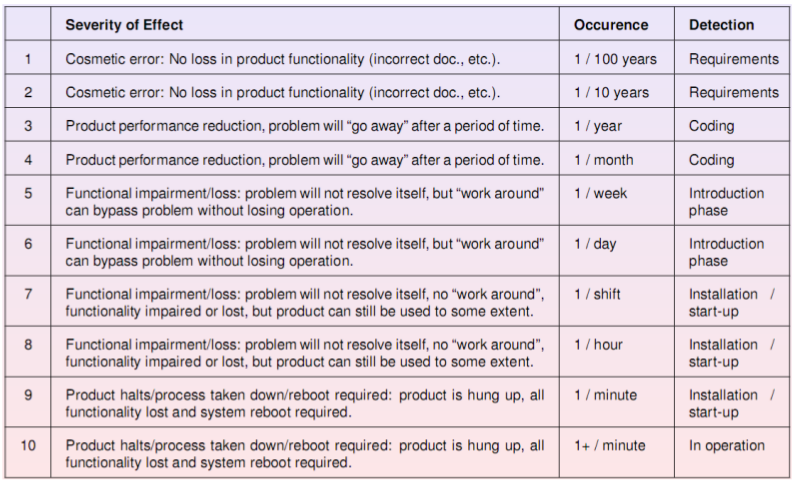
\includegraphics[width=1\textwidth]{img/fmea.png}



\section{Quellen}
\begin{table}[h]
\label{tab_quellen}
\begin{tabular}{llll}
{\textbf{Referenz}} & {\textbf{Vollnachweis}} 							\\
1 		&  Anderson, Shaun (2016). How Fast Should A Website Load. \\
		& http://www.hobo-web.co.uk/your-website-design-should-load-in-4-seconds/ \\
		& (01.04.2016). \\
		
2, 4 	&  Ackermann, Urs. 2015. Betriebswirtschaftslehre 2. S.208.\\

3 		& RA Rigert, Christian und MLaw Seger, Alice (2013). Rechtlichen Aspekte der \\
		& elektronischen Datenaufbewahrung. http://www.dieadvokatur.ch/fileadmin/ \\
		& user\_upload/Publikationen/Fachartikel/2013/Die\_rechtlichen \_Aspekte\_der\_ \\
		& elektronischen\_Archivierung.pdf (01.04.2016).\\

\end{tabular}
\end{table}

\chapter{Index}





\end{document}